\chapter{Aufbau der Webapplikationen}

\section{Framework für Graphalgorithmen}

Die Webapplikationen wurden in Analogie zu anderen, bereits bestehenden Applets für die Visualisierung verschiedener Graphalgorithmen konzeptioniert. Diese sind frei zugänglich auf der Webpräsenz des Lehrstuhls M5 für Mathematik an der TUM, erreichbar unter \href{https://www-m9.ma.tum.de/Allgemeines/GraphAlgorithmen}{https://www-m9.ma.tum.de/Allgemeines/GraphAlgorithmen}. 

Die bestehende Sammlung an Applets enthält bereits verschiedene andere Algorithmen der Graphentheorie, von Lösungsmethoden für des kürzeste Wege, Matchings, Spannbäume und mehr. Alle Anwendungen sind mit den gleichen Zielen entwickelt, die Algorithmen möglichst anschaulich und verständlich zu präsentieren, und verwenden das gleiche Seitenlayout. Auch die hier vorgestellten Applets zur Darstellung des Ford-Fulkerson Algorithmus und des Cycle Canceling Algorithmus stellen die Informationen in diesem bewährten Layout dar. Die Inhalte sind auf mehrere Tabs verteilt, die verschiedene Materialien bieten.

\paragraph{Tab: Einführung}

Die erste Einführung für den Benutzer gibt einen kurzen Überblick über die Problemstellung, die mithilfe des Algorithmus gelöst wird.
\begin{center}
\begin{minipage}[t]{0.80\textwidth}
    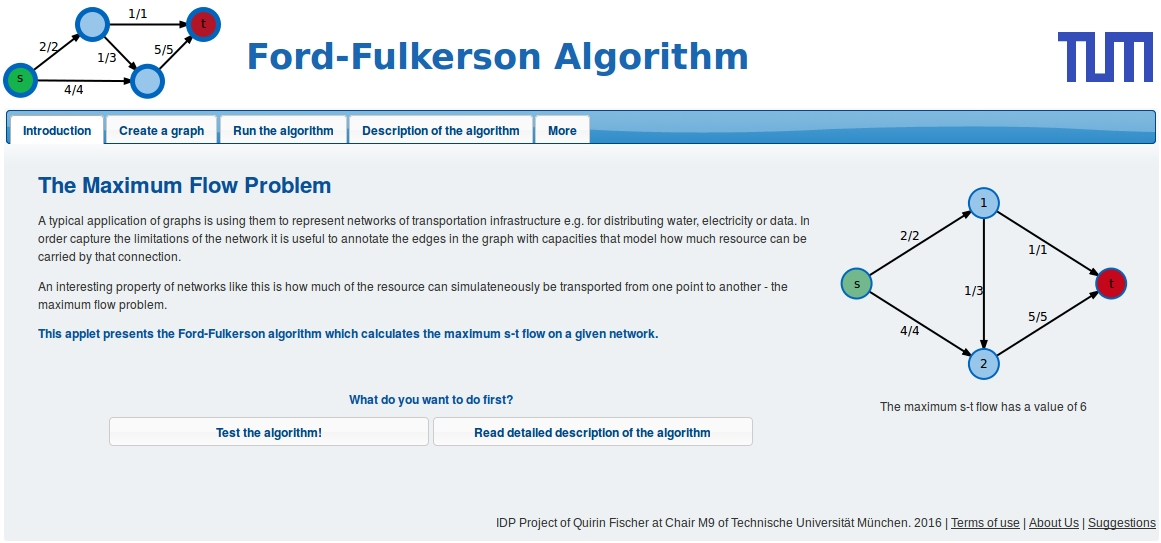
\includegraphics[width=\textwidth]{img/layout-1.jpg}
    \captionof{figure}{Der Einführungs-Tab.}
\end{minipage}
\end{center}
\vspace{1cm}

\paragraph{Tab: Grapherstellung} Ein Grapheditor, um die Instanz des Problems auszuwählen, auf der der Algorithmus ausgeführt werden soll. Der Editor bietet sowohl die Möglichkeit, vorgefertigte Beispiele zu laden, als auch diese zu verändern oder eigene Instanzen anzulegen. Knoten und Kanten des Graphen können einfach angelegt und gelöscht werden, und auf Klick ist auch die Modifikation zusätzlicher Eigenschaften wie Kantengewichte oder Kapazitäten möglich.

\begin{center}
\begin{minipage}[t]{0.60\textwidth}
    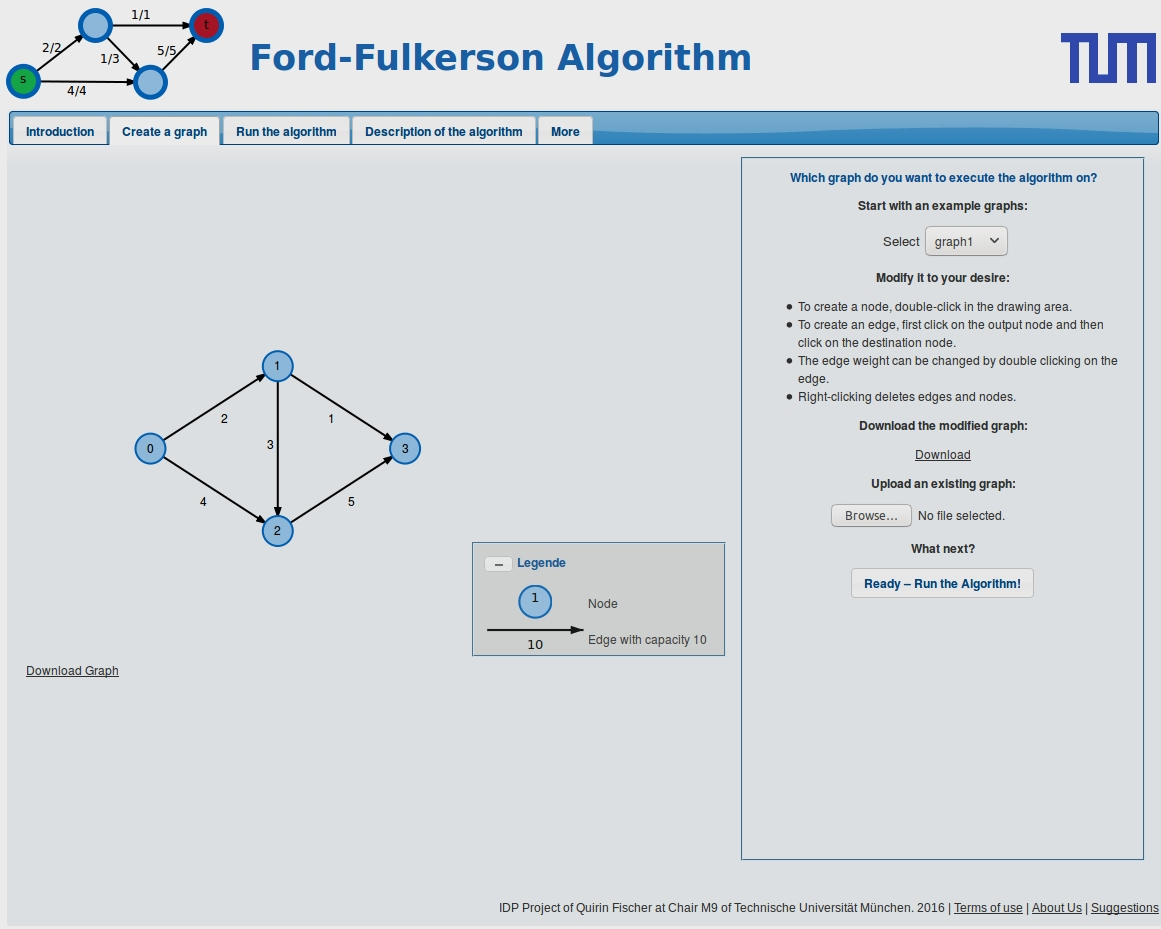
\includegraphics[width=\textwidth]{img/layout-2.jpg}
    \captionof{figure}{Der Tab des Grapheditors.}
\end{minipage}
\end{center}
\vspace{1cm}

\paragraph{Tab: Ausführung Algorithmus}

Der wichtigste Tab erlaubt die schrittweise Ausführung des Algorithmus und zeigt die internen Datenstrukturen. Einige Informationen werden grafisch in die Darstellung des Graphen integriert, indem beispielsweise Knoten oder Kanten farblich hervorgehoben werden. Eine seitliche Anzeige liefert wahlweise eine textuelle Beschreibung des aktuellen Arbeitsschrittes, die aktuelle Ausführungsposition in einer Pseudocode-Diagramm, oder die Werte von Variablen die der Algorithmus verwendet.

Die darzustellenden Daten unterscheiden sich zwischen den Algorithmen, so dass die Applikationen sich in diesem Tab am deutlichsten unterscheiden.

\begin{center}
\begin{minipage}[t]{0.60\textwidth}
    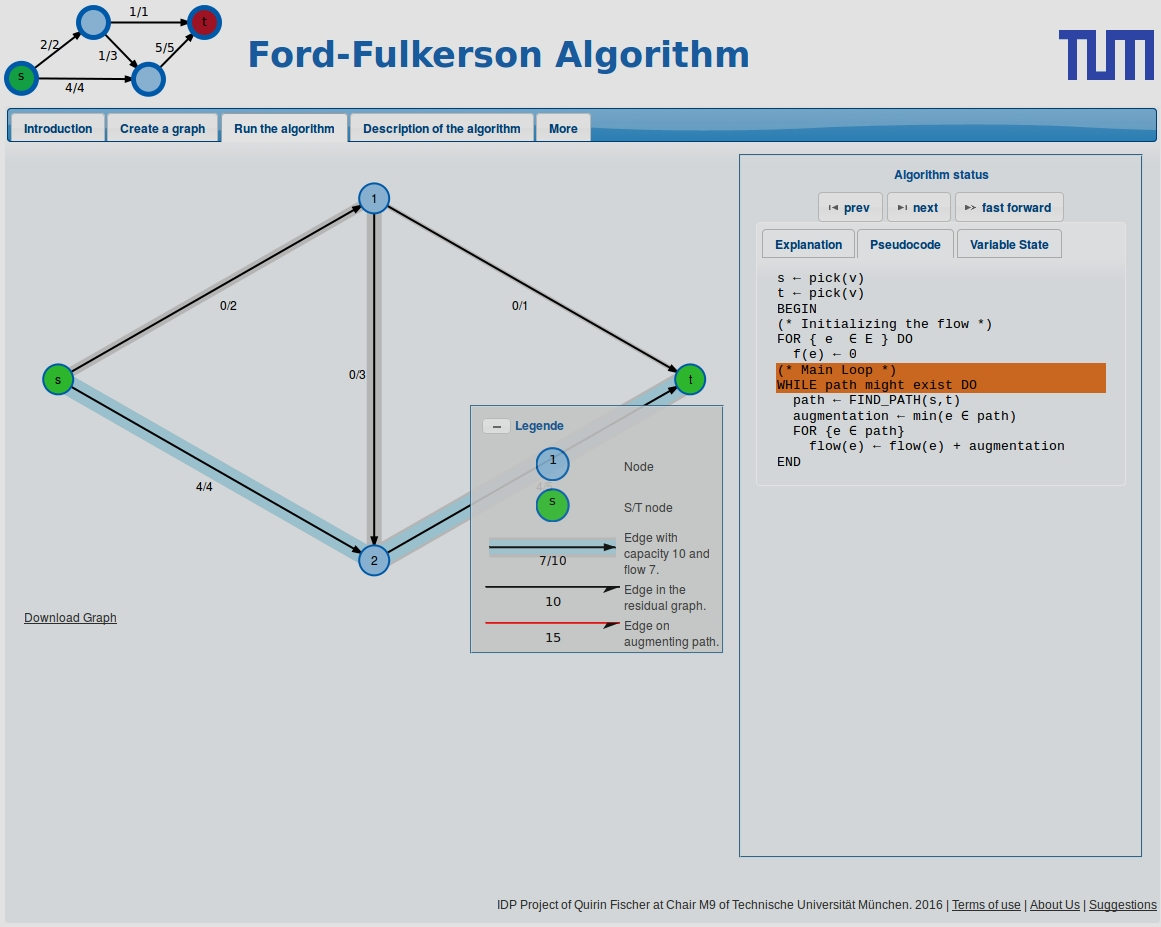
\includegraphics[width=\textwidth]{img/layout-3.jpg}
    \captionof{figure}{Der Algorithmus-Tab erlaubt schrittweise Ausführung und visualisiert den Status.}
\end{minipage}
\end{center}
\vspace{0.7cm}

\paragraph{Tab: Beschreibung Algorithmus}

Eine ausführlichere Beschreibung erläutert die Problemstellung und den genauen Ablauf des Algorithmus.

\begin{center}
\begin{minipage}[t]{0.60\textwidth}
    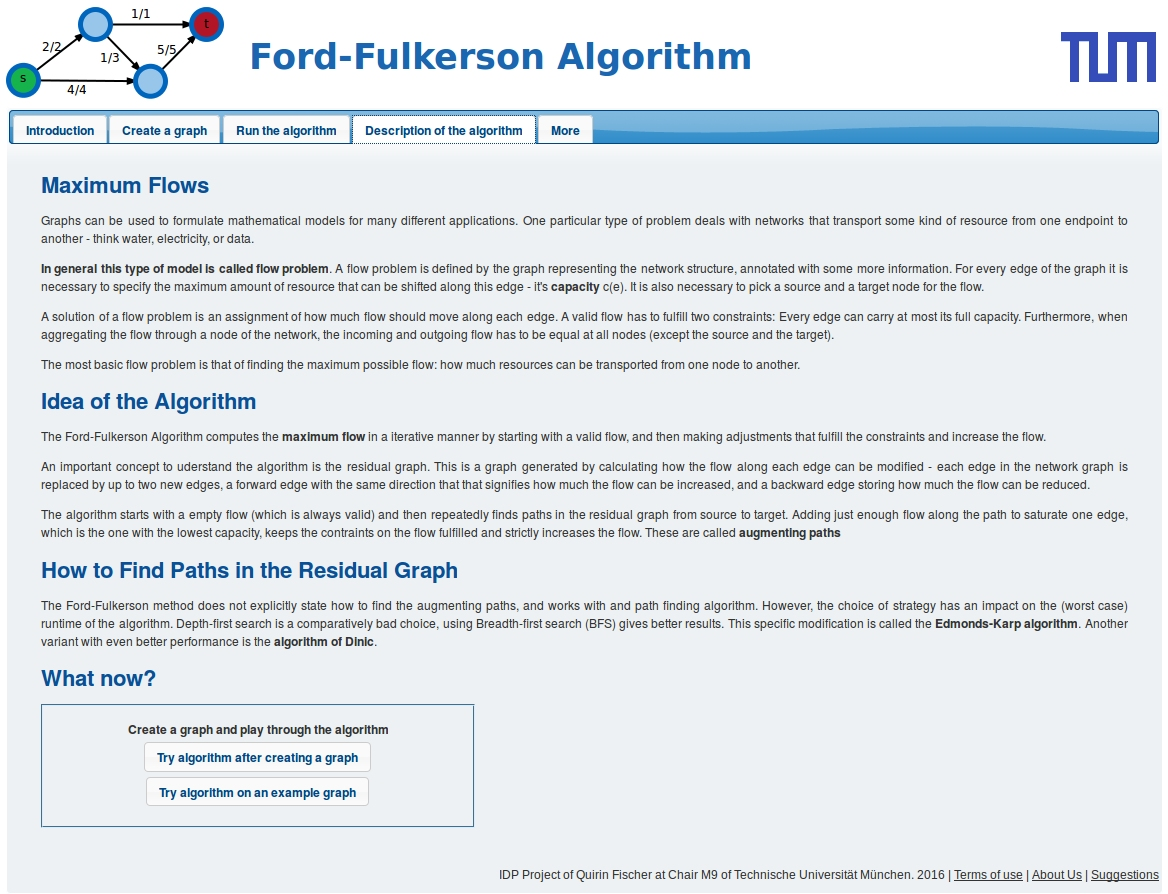
\includegraphics[width=\textwidth]{img/layout-4.jpg}
    \captionof{figure}{Eine längere Beschreibung des Algorithmus befindet sich im vierten Tab.}
\end{minipage}
\end{center}
\vspace{1cm}

\paragraph{Tab: Weitere Informationen}

Eine Sammlung nützlicher Informationen wie Beispielsweise einer Pseudocode-Darstellung des Algorithmus, Informationen zur Effizienz des Algorithmus, Hinweise auf abgewandelte Varianten oder eine Auswahl an Literatur und Referenzen.

\begin{center}
\begin{minipage}[t]{0.60\textwidth}
    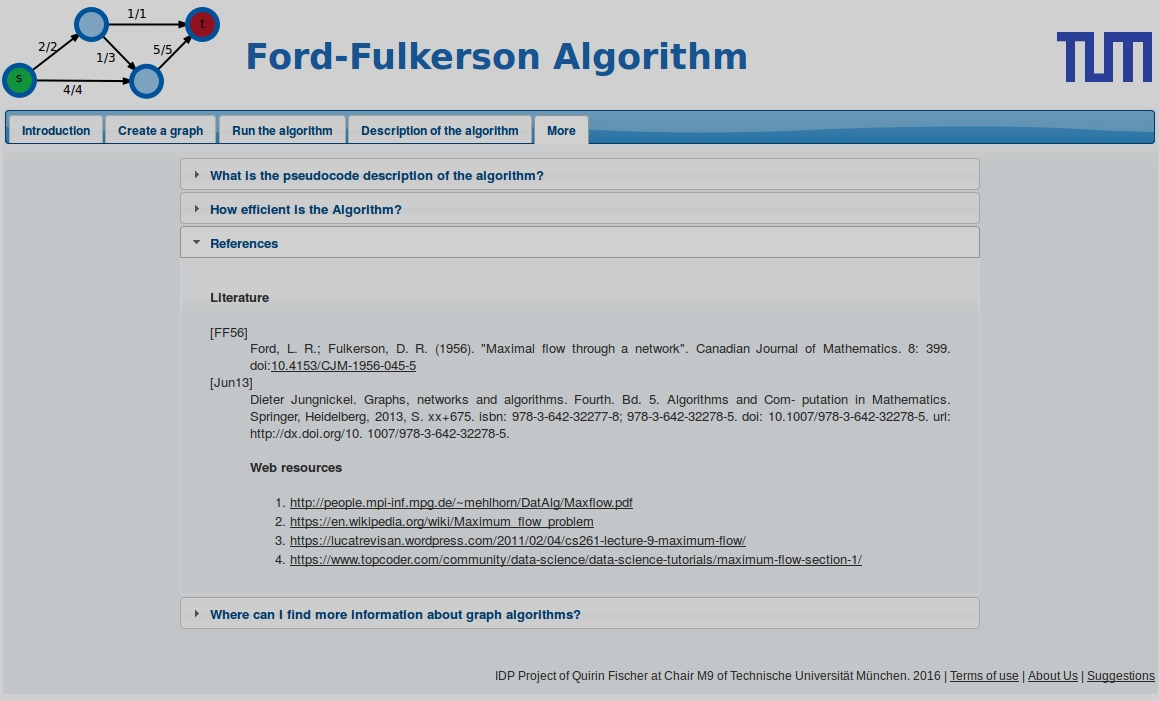
\includegraphics[width=\textwidth]{img/layout-5.jpg}
    \captionof{figure}{Der letzte Tab enthält weiteres Hintergrundmaterial.}
\end{minipage}
\end{center}


\section{Visualisierung des Ford-Fulkerson Algorithmus}

Während der Ausführung des Ford-Fulkerson Algorithmus verändert sind vor allem der Inhalt dreier Datenstrukturen: der aktuelle Fluss, das zugehörige Residualnetz, und sofern vorhanden der aktuelle augmentierende Pfad. Der Algorithmus alterniert Änderungen an diesen Daten - zunächst ist ein Fluss vorhanden, ausgehend von diesem wird das Residualnetz bestimmt, die Pfadsuche ergibt einen augmentierenden Pfad, woraufhin bei einem neuen Fluss begonnen wird. Die Visualisierung reflektiert diesen Ablauf und wechselt zwischen drei verschiedenen Ansichten.

In der ersten Ansicht wird ein Fluss visualisiert, indem die Kapazitäten und Flüsse der Kanten durch farbige Umrandung in verschiedenen Stärken dargestellt werden. Ein grauer Farbton zeigt freie Kapazität an, und eine helleres Blau zeigt vorhandenen Fluss. Diese Farbkodierung signalisiert klar, über welche Kanten der Fluss verläuft und wo sich freie Kapazität befindet.

Die zweite Ansicht zeigt das Residualnetzwerk des aktuellen Flusses. Die Richtungen der verfügbaren Kanten (oder der zugehörigen Rückkanten) werden durch Pfeilspitzen gekennzeichnet, mit Angabe der verfügbaren Kapazität auf der entsprechenden Seite der Kante. In der dritten Ansicht wird in diesem Netz der augmentierende Pfad farblich stark hervorgehoben, indem die Kanten des Pfades rot eingefärbt werden.

\begin{center}
\begin{minipage}[t]{0.58\textwidth}
    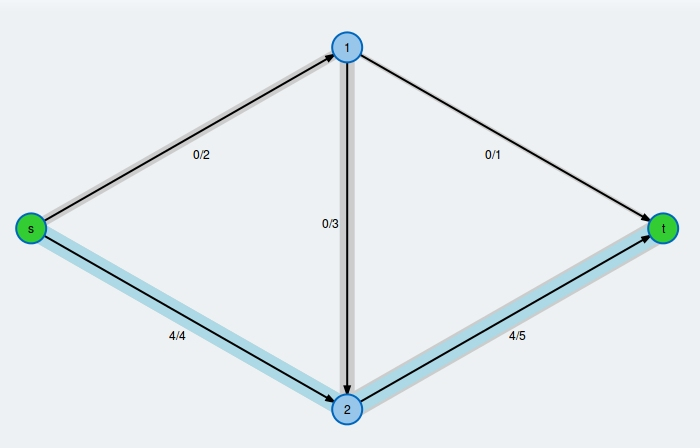
\includegraphics[width=\textwidth]{img/ford-fulkerson-1.jpg}
    \captionof{figure}{Flüsse und freie Kapazitäten werden farblich signalisiert.}
\end{minipage}
\end{center}


\begin{center}
\begin{minipage}[t]{0.58\textwidth}
    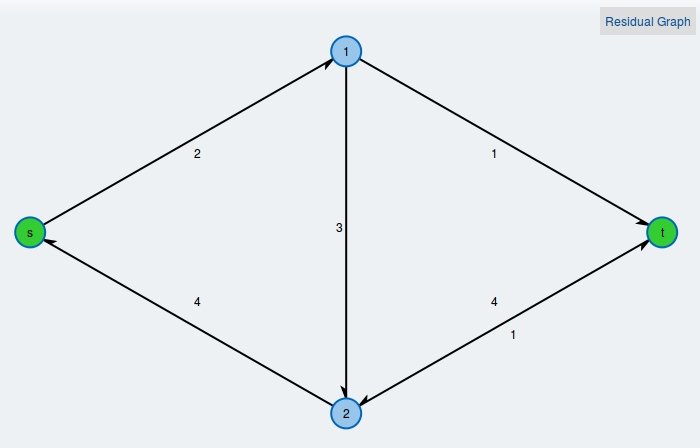
\includegraphics[width=\textwidth]{img/ford-fulkerson-2.jpg}
    \captionof{figure}{Das entsprechende Residualnetz.}
\end{minipage}
\end{center}


\begin{center}
\begin{minipage}[t]{0.58\textwidth}
    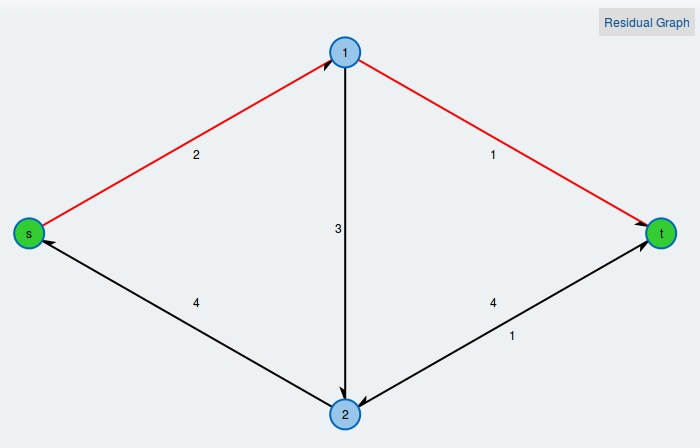
\includegraphics[width=\textwidth]{img/ford-fulkerson-3.jpg}
    \captionof{figure}{Der augmentierende Pfad wird rot gekennzeichnet.}
\end{minipage}
\end{center}


\section{Visualisierung des Cycle Canceling Algorithmus}

Auch der Cycle Canceling Algorithmus alterniert zwischen der Anzeige des aktuellen Flusses, des Residualnetzwerks, und des Residualnetzes mit hervorgehobenem negativen Kreis. Im Unterschied zum Ford-Fulkerson Algorithmus werden allerdings bei der Anzeige des Flusses zusätzlich die Kosten der Kanten angezeigt. Im Residualnetz sind die Kanten mit ihren Kosten beschriftet und nicht mit den Kapazitäten, da diese bei der Kreiserkennung verwendet werden. Die Visualisierung verwendet das gleiche Farbschema, negative Kreise werden also ebenfall in rot hervorgehoben.

\begin{center}
\begin{minipage}[t]{0.70\textwidth}
    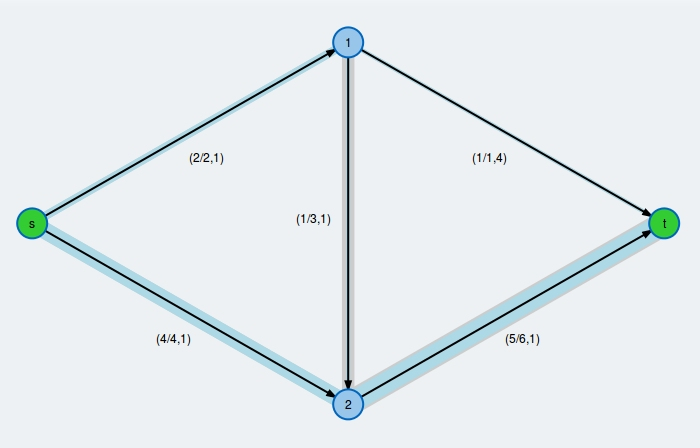
\includegraphics[width=\textwidth]{img/cycle-canceling-1.jpg}
    \captionof{figure}{Flüsse und freie Kapazitäten werden farblich signalisiert, mit zusätzlicher anzeige der Kosten.}
\end{minipage}
\end{center}


\begin{center}
\begin{minipage}[t]{0.70\textwidth}
    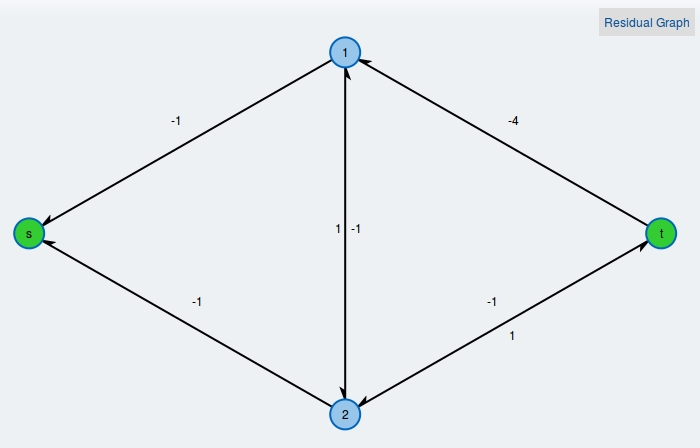
\includegraphics[width=\textwidth]{img/cycle-canceling-2.jpg}
    \captionof{figure}{Im Residualnetz sind die Kanten mit ihren Kosten beschriftet.}
\end{minipage}
\end{center}


\begin{center}
\begin{minipage}[t]{0.70\textwidth}
    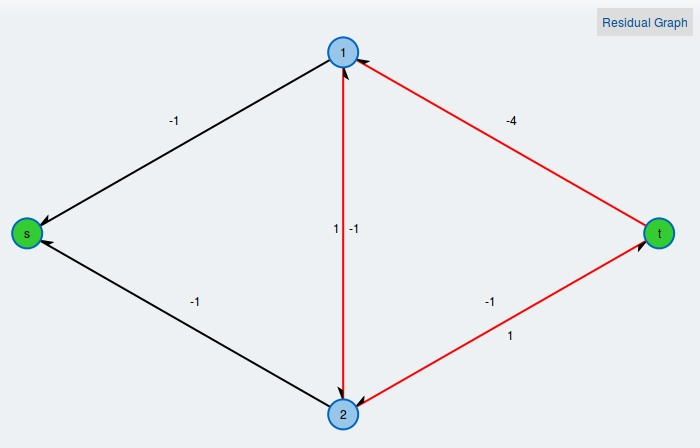
\includegraphics[width=\textwidth]{img/cycle-canceling-3.jpg}
    \captionof{figure}{Ein erkannter negativer Kreis wird in rot markiert.}
\end{minipage}
\end{center}
